\chapter[SCP-121 混凝土摇篮]{
    SCP-121 Concrete Cradle\\
    SCP-121 混凝土摇篮
}

\label{chap:SCP-121}

\begin{figure}[H]
    \centering
    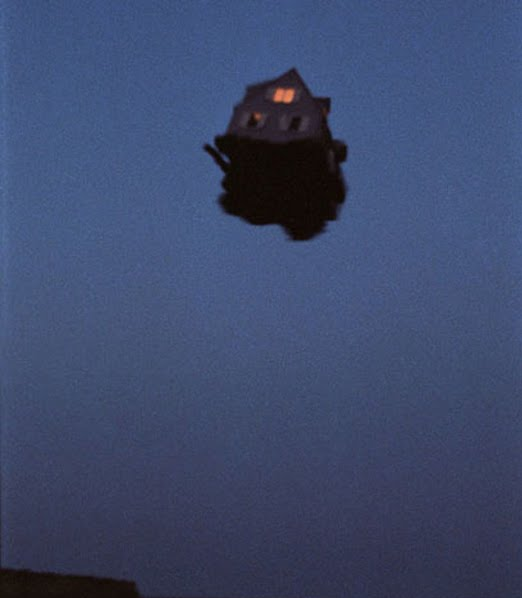
\includegraphics[width=0.5\linewidth]{images/SCP.121.png}
    \caption*{活化中的 SCP-121-1实体}
\end{figure}

\bb{项目编号:}SCP-121

\bb{项目等级:}Euclid

\bb{特殊收容措施:}Site-83建立在SCP-121外部,供那些致力于收容SCP-121的研究人员使用。SCP-121的影响范围一直处于对外隔离状态,并有警卫站驻扎。警卫身着当地军队制服,时刻全副武装,每4小时换班轮值。

周边区域的普通居民都已保持获悉SCP-121是一片疫情隔离区,在不停释放有害物质。所有通往SCP-121的道路在距离项目地点七十五(75)、五十(50)、二十五(25)公里处都设有明令警告牌,旨在阻拦入侵者。那些接近SCP-121边界的平民将被告知该地段正处于疫情隔离状态,必须立即远离;凡是违反禁令不愿离开的,将因其质疑态度或滞留行为而遭到人身扣押。

一旦发生有平民接近且目击SCP-121-1或-2事件,需对目击者执行A级记忆消除。任何因SCP-121反常特性导致气象变化所产生的记录需在审查后删除,且为了防止SCP-121,-1,-2的相关信息外泄,SCP-121已被列为禁飞区。

站点特遣部队Iota-71“小鬼当家”(Home Wreckers),已成功建制并长期驻守Site-83收容所,专责应对SCP-121-2所造成的威胁。他们负责护送对SCP-121-2感兴趣的科学家研究其无威胁状态,并在其产生具有潜在致命体积的实体时,使用中和手段消除威胁。在尝试突破收容控制的突发事件中,Iota-71将协助边界警卫一同中和SCP-121-2实体。

任何SCP-121范围内的建筑如果演化成SCP-121-1,必须被记录在案并且实行24小时不中断监控,以防转变为SCP-121-2。那种天生带有敌意的SCP-121-2必须被中和;然而,一些消极被动的实体被允许保留在SCP-121戒严范围内并被用于研究,直到其成长为继续收容会产生一定危险的体积,或是产生了敌意,无论哪一种情况它都将被中和。

\bb{描述:}SCP-121位于科罗拉多州,是一片隶属于███████镇的土地。在达成收容协定之前,粗略估计该小镇曾经拥有6800位居民,3000座住宅或商业建筑。在SCP-121上方的天空中,有一块直径达到约十二(12)千米的禁区,路过的云团无法进入,只能选择从旁飘过;据推测,这片区域与SCP-121的影响范围有关,但时至今日,研究人员尚未找到一个明确的答案。在SCP-121范围内的建筑群能够极个别地\footnote{在同一时期只有一座建筑会悬浮,两次升空现象之间至少有三周间隔期。}从地面分离并飘至半空,此时,这些升空建筑将被定义为SCP-121-1。

SCP-121-1实体会上升到一个至少四十五(45)米高的随机高度。无论该建筑之前的状态如何,升空后的门窗都将上锁,任何入侵行为都会被其内部家具阻挡。暴力破开闯入则会导致环境温度上升至35℃,相对湿度达到65\%,但缺乏任何进一步的异常反应。SCP-121-1实体的悬浮期将至少保持10周,一般不超过15周。SCP-121-1实体的耐久度并无任何异常,几乎所有常见的破坏现象都是由跌落导致。在落地后,SCP-121-1实体的废墟中往往包含一种大小约1.2m x 1.2m x 2m,由家具材料组成的卵状生物\footnote{针对大部分保存完好的SCP-121-1进行检查发现,缺少了一部分先前的家具。}。这种物体会根据自身意志移动;此时,该物体被定义为SCP-121-2。

\begin{figure}[H]
    \centering
    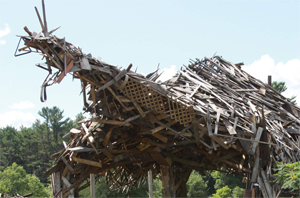
\includegraphics[width=0.5\linewidth]{images/SCP.121.2.png}
    \caption*{成长中的 SCP-121-2实体}
\end{figure}

SCP-121-2会开始利用周边材料包裹自身,从而组成某种集合体,这些材料包括SCP-121-1的残片、植物、汽车,以及(罕见情况下)其他建筑物\footnote{这种现象很偶然,当新生的SCP-121-1建筑离SCP-121-2相当近时才会发生。}。

SCP-121-2将持续吸附物质,直到其身体组成达到九(9)米高度时,它将活化并表现出对外界具有一定程度的探知能力。此后,SCP-121-2可能出现像是摄取、吸收、消化其他材料的行为,以相当慢的速度继续增长。如果实体在相当长的一段时间里没有进食,这种摄取行为便成了其继续维持增长的唯一目的。已知有好几种物品能够瞬间被SCP-121-2吸附,无论其体积大小,以及该实体是否处于模拟摄食状态。

SCP-121-2实体的外形通常会模仿一些陆行动物,也有少数模仿出了类人型生物,但并没有任何一种外貌与现存动物完全相同。它们通常很温顺,并不会表现出敌意行为,除非被激怒。然而,已知部分SCP-121-2实体天生具有敌意和领地意识行为;经观察,这种行为的出现似乎与特定物品的吸附积累有关,包括各种枪炮、刀剑,以及某次特例:一颗动物标本熊头。

当地方政府收到许多有关废弃房屋“在天上飞”的报告时,SCP-121开始被基金会关注。在有毒物质泄露的幌子遮盖下,整个小镇的居民都被疏散撤离。当一个SCP-121-1实体开始转型成为SCP-121-2时,原有的SCP-121-2便会迅速进入中和期,变得失活并无效化。紧接着,在这种中和反应之后,新的SCP-121-1实体会开始产生,整个小镇已经永久撤离并被收容保护。

\bb{事件121-A:}1998年11月4日,一阵“低沉的汽笛”之音持续了约莫五(5)分钟。伴随着这声响动,一件悬浮时间并未达到十周最短期限的SCP-121-1实体在某种巨大力量的影响下,直接于空中解体。临近城镇报道了这次异动;当地媒体获悉,因有毒物质的产生突然出现临时性增加,检疫工作人员被迫撤离。造成声响的原因至今未明,建议进一步研究。

在怪响发生以及SCP-121-1裂解三周后,这座四分五裂的建筑终于落地。其残骸内发现的卵形对象SCP-121-2正躺在一堆铝渣中\footnote{汽笛爆鸣、巨力裂解、残留铝渣……综合起来可能是某种涉及到大型铝热反应的情形——译者注}。

\bb{事件121-B:}2012年5月9日,一辆1991年产道奇凯领\footnote{1991 Dodge Caravan,一款道奇牌厢式商务车——译者注}被发现悬浮于五十三(53)米高的空中。因为其全部车窗似乎都被一种羊毛布料所遮挡,从外面无法监控到车辆内部情况。建议进一步观察该车辆。
